%!TEX root = these.tex

\chapter{Review of runtime verification and related work}

In this chapter, we firstly review the common information of runtime verification, including the history, the definition and the comparison with other verification techniques. Secondly, linear temporal logic, as the common specification formalism of runtime verification, is presented with the syntax, the operators and the semantics. At last, a few well-known runtime verification frameworks are introduced, as well as a simple comparison of them.

\section{Runtime verification}

\subsection{Conception}

Software verification and validation, as an important aspect of project management and software engineering, is the process of employing various necessary techniques to detect the violations or satisfactions and to evaluate the software quality and the performance of a system \citep{ieeestd2012}.

There are normally two kinds of verification techniques: static and dynamic analysis. Some well-knowns traditional techniques of static analysis are model checking \citep{clarke1999model} and theorem proving \citep{heisel1990tactical}. Static analysis is usually applied to verify the behaviors of a system before its execution, but such techniques have natural shortcomings. For example, model checking cannot work on a system of which the size or the number of states might grow beyond the capacity of computational power owing to the ``state-explosion problem''.

Dynamic analysis is to monitor running systems. Although sometimes its result might be false negatives because of its incompleteness, this incompleteness enables the techniques of dynamic analysis to break the limitation of static methods and thus become their complementary verification
methods. \citep{falcone2013tutorial}

Runtime verification (RV) is a kind of verification technique based on dynamic analysis. In 2001, the Runtime verification workshop \footnote{http://www.runtime-verification.org/} was founded, as the terminology ``runtime verification'' was officially introduced \citep{wiki:rv}. It is a relatively new technique which is lightweight and aims to complement other traditional verification techniques like model checking and testing.

\cite{leucker2009brief} defines runtime verification as follows:
\begin{displayquote}
Runtime verification is the discipline of computer science that deals with the study, development, and application of those verification techniques that allow checking whether a run of a system under scrutiny satisfies or violates a given correctness property.
\end{displayquote}

Normally when a violation is observed, runtime verification does not fix the detected program itself, but its result is an important guide and basis for other component in the same system to deal with the problem.

\cite{leucker2009brief} also defines a \emph{run} of a system as a sequence of infinite traces of the system, and an \emph{execution} of a system as a finite trace and also a \emph{finite prefix} of a \emph{run}. The work of runtime verification mainly focuses on the analysis of \emph{executions} which are performed by \emph{monitors}.

A \emph{monitor} is a decision procedure generated (or ``synthesized'') from one of the formal properties which is to be verified against the execution of the given system. During verification, a \emph{monitor} enumerates the finite traces of an \emph{execution}, checks whether they satisfy the correctness properties and produces a \emph{verdict} as the result. A \emph{verdict}, which is normally a truth value, indicates the satisfaction of the property against the gathered events.

A verdict in most simple cases normally can be expressed as true/value, yes/no or 1/0, depending on the context. But actually many runtime verification systems have to introduce other values to provide a more accurate result. For example, thanks to the incompleteness of runtime verification system, a verdict cannot be easily issued when the monitor needs more successive events, so a \emph{inconclusive} (written as ``?'') value is introduced to indicate the current status of the monitored system. \citep{falcone2013tutorial}

\subsection{Procedure}

\begin{figure}[h]
\begin{center}
\centering
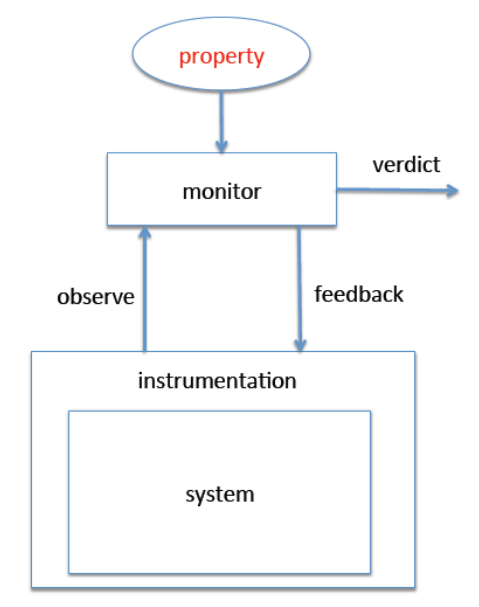
\includegraphics[width=80mm]{rvstruct.png}
\caption{Runtime verification process (from \cite{falcone2013tutorial})}
\label{img:rvstruct}
\end{center}
\end{figure}

Figure \ref{img:rvstruct} describes the process of a typical runtime verification system which contains the following four steps \citep{falcone2013tutorial}:
\begin{enumerate}
\item \emph{Monitor synthesis}: A monitor is synthesized from a property.
\item \emph{System instrumentation}: Extra instruments are integrated with the system under scrutiny in order to generate the events for the \emph{monitor}.
\item \emph{Execution}: The system is executed and starts to generate events and send them to the monitor.
\item \emph{Analysis and response}: The monitor analyzes the collected events, emits a \emph{verdict} and sends additional information, i.e. \emph{feedback} to the system if necessary.
\end{enumerate}

Monitors can be classified into several modes from different aspects \citep{chen2007mop}:
\begin{itemize}
\item \emph{online/offline} depends on when the monitors and the system work. \emph{Online} if they work at the same time, and \emph{offline} if the monitors start to work after the termination of the execution of the system.
\item \emph{inline/outline} depends on where the monitors are executed. \emph{inline} if the monitors are embedded into the system and \emph{outline} if the monitors run all alone while receiving the event traces from the system by certain methods, e.g. via file system or wireless signal.
\item \emph{violation/validation} is determined by the specification of the verdict.
\end{itemize}

From the definitions of the modes, we can see that a monitor working in offline mode is also working in outline mode and the inline mode implies the online mode.

\subsection{Comparison with other techniques}

Comparing with model checking \citep{clarke1999model} which aims to verify finite state systems, the methods of generating monitors in runtime verification and generating automatas in model checking have similarities. However, whereas model checking deals mainly with infinite traces, runtime verification deals only with finite traces, i.e. the executions. For this reason, the monitors of runtime verification working in online monitoring mode have to be able to accept incremental traces.

Another important difference between model checking and runtime verification is that, unlike model checking which checks if all executions of a system satisfy a correctness property, runtime verification is interested only with whether existing an execution which belongs to a set of valid executions. Moreover, runtime verification only requires to analyze the observed events of a given system without having to watch its internal running information, but in model checking, the proper model of the system must be acknowledged in order to prepare every possible execution before running the system. \citep{leucker2009brief}

Software testing \citep{broy2005model} is another verification technique. It is a process of running a program with a finite set of input-output sequences which is also namely test suite. Comparing with runtime verification, test suites are defined directly, unlike properties of runtime verification which are generated from formalism specification. Besides, ``exhaustive testing'' which is a common method in software testing, is normally not an option of runtime verification.

\section{Linear temporal logics}

In runtime verification, a monitor is translated from a correctness property, and correctness properties are specified in linear-time temporal logics, such as LTL.

Temporal logic is an extension of classical logic, and it provides a convenient language with the expressions of the properties to reason about the change of the states in terms of time. Although there are a lot of different temporal logics invented to meet various requirements, the temporal logics are normally classified by whether the time is linear or branching. The temporal logic with linear time is called \emph{Linear Temporal Logic} (LTL) which was first proposed by \cite{pnueli97}. Time in LTL is turned into a sequence of states which extend to the infinite future. The sequence of states is a computation \emph{path}. \citep{clarke1999model} \citep{huth2004}

\cite{leucker2009brief} summarizes LTL as a well-accepted linear-time temporal logic used to specify properties of infinite traces. However, in runtime verification, LTL is employed to check finite executions.

\subsection{Syntax}

A well-formed \emph{LTL} formula consists of a finite set of atomic propositions, boolean operators $\neg, \wedge, \vee, \rightarrow$ and temporal logic operators \textbf{F}(future), \textbf{G}(global), \textbf{X}(next), \textbf{U}(until), \textbf{W}(weak-until) and \textbf{R}(release). It can be represented in the Backus Naur form as follows \citep{huth2004}:
\begin{align}
\phi ::= & \top | \bot | p | (\neg\phi) | (\phi \wedge \phi) | (\phi \vee \phi) | (\phi \rightarrow \phi) \nonumber \\
& | (\X \phi) | (\F \phi) | (\G \phi) | (\phi \U \phi) | (\phi \W \phi) | (\phi \R \phi)
\end{align}

\subsection{Semantics}

For a sequence of states $s_0, s_1, s_2, ..., s_i, s_{i + 1}, ...$ where $s_{i + 1}$ is a future state of $s_i$, we define a path with $\pi^i = s_i \rightarrow s_{i + 1} \rightarrow ...$ where $i$ is the first state in this path. Given that $\pi(i)$ is the set of atomic propositions which are true at the $i$th state, whether a path $\pi^i$ satisfies an \emph{LTL} formula is defined as follows \citep{rozier2011linear}:

\begin{itemize}
  \item \listequation{\pi^i \vDash \top} \label{eq:true}
  \item \listequation{\pi^i \nvDash \bot} \label{eq:false}
  \item \listequation{\pi^i \vDash p \iff p \in \pi(i)} \label{eq:ap}
  \item \listequation{\pi^i \vDash \neg\psi \iff \pi^i \nvDash \psi} \label{eq:not}
  \item \listequation{\pi^i \vDash \psi \wedge \varphi \iff \pi^i \vDash \psi \text{ and } \pi^i \vDash \varphi} \label{eq:and}
  \item \listequation{\pi^i \vDash \psi \vee \varphi \iff \pi^i \vDash \psi \text{ or } \pi^i \vDash \varphi} \label{eq:or}
  \item \listequation{\pi^i \vDash \psi \rightarrow \varphi \iff \pi^i \vDash \varphi \text{ whenever } \pi^i \vDash \psi} \label{eq:then}
  \item \listequation{\pi^i \vDash \X \psi \iff \pi^{i + 1} \vDash \psi} \label{eq:next}
  \item \listequation{\pi^i \vDash \G \psi \iff \forall j \geq i, \pi^j \vDash \psi} \label{eq:global}
  \item \listequation{\pi^i \vDash \F \psi \iff \exists j \geq i, \pi^j \vDash \psi} \label{eq:future}
  \item \listequation{\pi^i \vDash \psi \U \varphi \iff \exists j \geq i, \pi^j \vDash \varphi$ and $\forall k, i \leq k < j, \pi^k \vDash \psi} \label{eq:until}
  \item \listequation{\pi^i \vDash \psi \W \varphi \iff$ either $\exists j \geq i, \pi^j \vDash \varphi$ and $\forall k, i \leq k < j, \pi^k \vDash \psi$, or $\forall k \geq i, \pi^k \vDash \psi} \label{eq:wuntil}
  \item \listequation{\pi^i \vDash \psi \R \varphi \iff$ either $\exists j \geq i, \pi^j \vDash \psi$ and $\forall k, i \leq k \leq j, \pi^k \vDash \varphi$, or $\forall k \geq i, \pi^k \vDash \varphi} \label{eq:release}
\end{itemize}

Formul\ae{}s \ref{eq:true} and \ref{eq:false} suggest that the states in the path $\pi^i$ should be always true or false.

In formul\ae{} \ref{eq:ap}, $p$ is an atomic proposition belonging to the finite set of atomic propositions of LTL, and this formul\ae{} demands to check only the $i$th state.

Formul\ae{}s \ref{eq:not}---\ref{eq:then} are boolean operators of propositional logic following the rules of Table \ref{table:prologic}

\begin{table}[h]
\centering
\begin{tabular}{|c|c|c|c|c|c|}
\hline
$\psi$ & $\varphi$ & $\neg\psi$ & $\psi \wedge \varphi$ & $\psi \vee \varphi$ & $\psi \rightarrow \varphi$ \\
\hline
True & True & False & True & True & True \\
\hline
True & False & False & False & True & False \\
\hline
False & True & True & False & True & True \\
\hline
False & False & True & False & True & True \\
\hline
\end{tabular}
\caption{The truth table of boolean operators of propositional logic}
\label{table:prologic}
\end{table}

Formul\ae{}s \ref{eq:next}, \ref{eq:future} and \ref{eq:global} are unary temporal logic connectives.
\X means ``next time'' and it skips the $i$th state and evaluates the path $\pi^{i+1}$. \F stands for ``sometimes in the future'' which requires that from the $i$th state, a property holds in a future state on the path. And \G (``globally'' or ``always'') denotes that a property should hold on the every state from the $i$th state until the end or the infinite future.

Formul\ae{}s \ref{eq:until}, \ref{eq:wuntil} and \ref{eq:release} are binary temporal logic operators. \U is the abbreviation of ``until''. The formul\ae{} $\psi \U \varphi$ holds if $\varphi$ holds at a future state on the path, and before this state the property $\psi$ holds at every state. \W, ``weak-until'', is a weak version of \U, except that for the formul\ae{} $\psi \W \varphi$, $\varphi$ does not have to hold eventually in some future state. \R, which stands for ``release'', is actually a logic dual of \U, i.e. $\psi \U \varphi \equiv \neg(\neg\psi \R \neg\varphi)$. \R requires that for the formul\ae{} $\psi \R \varphi$, the property $\varphi$ should hold continuously until $psi$ holds or $psi$ does not hold eventually.

It is worth noting that in LTL, the two-valued logics might yield a premature result which is either true or false. As is mentioned above, LTL is defined to work with infinite traces whereas monitoring of runtime verification is only able to treat finite traces, which might lead to a conflict, especially in some running system. For instance, $\F \psi$ states that $\psi$ should hold in a future state. In a running system, as long as $\psi$ does not hold in the observed states, the results of the formul\ae{} are always $false$, but if $\psi$ holds in the next observation, the former results will become corrupted and obsolete. Therefore, \cite{bauer2006monitoring} proposed the three-valued logic LTL$_3$ which introduces an new value \emph{inconclusive} for the cases where the property cannot be evaluated immediately.

\subsection{Various LTLs}

\subsubsection{Metric Temporal Logic}

Metric Temporal Logic (MTL) \citep{chang1994compositional} was invented to reason about real-time properties. To precise time accurately, MTL cuts the time into numbered pieces which is also called timed transition modules, and employs boundary operators to constrain the temporal logic operators. Its formul\ae{} is defined as follows:
\begin{align*}
\phi ::= & \bot | p | (\phi \rightarrow \phi) | (\fullmoon_{\sim{}c}\phi) | (\circleddash_{\sim{}c}\phi) | (\phi \mathrel{U}_{\sim{}c} \phi) | (\phi \mathrel{S}_{\sim{}c} \phi) \\
& \mbox{where } \sim \in \{<, =, >, \equiv_d\} \mbox{ and } c \geq 0, d \geq 2
\end{align*}

$\fullmoon_{\sim{}c}\phi$ means ``Next'', $\circleddash_{\sim{}c}\phi$ means ``Previous'', $\phi \mathrel{U}_{\sim{}c} \phi$ means ``Until'' and $\phi \mathrel{S}_{\sim{}c} \phi$ means ``Since'' \citep{chang1994compositional}. Given that $T_i$ indicates the time of the $i$th state of the path $\pi^i$, whether a formul\ae{} holds at the position $j$ of the path $\pi$ is defined as follows (we ignore the propositional operators here):
\begin{eqnarray*}
\pi^i \vDash \fullmoon_{\sim{}c}\psi & \iff & \pi^{i+1} \vDash \psi \mbox{ and } T_{i+1} - T_i \sim c \\
\pi^i \vDash \circleddash_{\sim{}c}\psi & \iff & i \geq 1 \mbox{ and } \pi^{i-1} \vDash \psi \mbox{ and } T_i - T_{i-1} \sim c \\
\pi^i \vDash \psi \mathrel{U}_{\sim{}c} \varphi & \iff & \exists j \mbox{ where } i \leq j, \pi^j \vDash \varphi \mbox{ and } T_k - T_j \sim c, and \forall k \mbox{ where } i \leq k < j, \pi^k \vDash \psi \\
\pi^i \vDash \psi \mathrel{S}_{\sim{}c} \varphi & \iff & \exists j \mbox{ where } 0 \leq j \leq i, \pi^j \vDash \varphi \mbox{ and } T_j - T_k \sim c, and \forall k \mbox{ where } j < k \leq j, \pi^k \vDash \psi \\
\end{eqnarray*}

\subsubsection{Past time LTL}

Whereas LTL mentioned in the last part is defined to check the future states, Past time LTL (ptLTL) aims to verify the states in the past. A ptLTL formul\ae{} is defined as follows \citep{havelund2004efficient}:
\begin{align*}
\phi ::= & \top | \bot | p | (\neg\phi) | (\phi \wedge \phi) | (\phi \vee \phi) | (\phi \rightarrow \phi) \\
& | (\odot \phi) | (\diamond \phi) | (\boxdot \phi) | (\phi \mathrel{S_s} \phi) | (\phi \mathrel{S_w} \phi) \\
& | (\uparrow \phi) | (\downarrow \phi) | [\phi, \phi)_s | [\phi, \phi)_w
\end{align*}

As can be seen in the definition of the formul\ae{}, ptLTL keeps several basic operators as LTL and introduces five standard part time operators and four monitoring operators.

The five standard part time operators are $\odot $ which means ``previous'', $\diamond$ ``eventually in the past'', $\boxdot$ ``always in the past'', $\mathrel{S_s}$ ``strong since'' and $\mathrel{S_w}$ ``weak since''.

The monitoring operators $\uparrow \downarrow [,)_s [,)_w$ mean respectively ``start'', ``end'', ``strong  interval'' and ``weak  interval''.

The temporal operators' semantics are described as follows, in the same form of the last section:
\begin{eqnarray*}
\pi^i \vDash \odot \psi & \iff & \mbox{ if } i > 0, \pi^{i - 1} \vDash \psi, or \mbox{ if } i = 0, \pi^0 \vDash \psi \\
\pi^i \vDash \diamond \psi & \iff & i > 0 \mbox{ and } \exists j \mbox{ where } 0 \leq j \leq i, \pi^j \vDash \psi \\
\pi^i \vDash \boxdot \psi & \iff & i > 0 \mbox{ and } \forall j \mbox{ where } 0 \leq j \leq i, \pi^j \vDash \psi \\
\pi^i \vDash \psi \mathrel{S_s} \varphi & \iff & \exists 0 \leq j \leq i, \pi^j \vDash \varphi \mbox{ and } \forall k, j < k \leq i, \pi^k \vDash \psi \\
\pi^i \vDash \psi \mathrel{S_w} \varphi & \iff & \pi^i \vDash \psi \mathrel{S_s} \varphi \mbox{ or } \pi^i \vDash \boxdot\psi \\
\pi^i \vDash \uparrow \psi & \iff & \pi^i \vDash \psi \mbox{ and } \pi^{i - 1} \nvDash \psi \\
\pi^i \vDash \downarrow \psi & \iff & \pi^i \nvDash \psi \mbox{ and } \pi^{i - 1} \vDash \psi \\
\pi^i \vDash [\psi, \varphi)_s & \iff & \exists j \mbox{ where } 0 \leq j \leq i, \pi^j \vDash \psi, \mbox{ and } \forall k \mbox{ where } j \leq k \leq i, \pi^k \nvDash \varphi \\
\pi^i \vDash [\psi, \varphi)_w & \iff & \pi^i \vDash [\psi, \varphi)_s \mbox{ or } \pi^i \vDash \boxdot\neg\varphi \\
\end{eqnarray*}

\subsubsection{EAGLE}

EAGLE \citep{barringer2004rule} is a temporal finite trace monitoring logic supporting parameterized equations by combining minimal/maximal fix-point semantics with temporal operators.

Online runtime verification requires to accept incremental traces which means there are possible boundaries between traces. Minimal/maximal fix-point rules were designed to treat this problem. Before evaluating the next trace, the equations with maximal rules are required to be always right and the ones with minimal rules are only needed to be eventually right.

\section{Runtime verification frameworks}\label{sec:rv:frameworks}

In runtime verification, monitors are generated from formal specifications by runtime verification frameworks. There are four monitoring modes: offline, online, inline and outline as we discussed in the early part of this section. Many frameworks and systems using some variant or extension of LTL have been proposed, as Table \ref{table:rvframeworks} shows. 

\begin{table}[h]
\centering
\begin{tabular}{|c|c|c|}
\hline
Name & Logic & Mode \\
\hline
JPax\citep{havelund2001java} & LTL \& Past-time LTL & outline \\
\hline
JavaMaC\citep{kim2004java} & Past-time LTL & outline \\
\hline
Hawk \citep{d2005event} & Hawk & outline \\
\hline
Temporal Rover\citep{drusinsky2000temporal} & LTL \& MTL & outline \\
\hline
MOP \citep{chen2007mop} & Various & inline/outline/offline \\
\hline
\end{tabular}
\caption{Runtime Verification Frameworks}
\label{table:rvframeworks}
\end{table}

Java PathExplorer (JPaX) \citep{havelund2001java} is an online runtime verification system aiming to monitor the execution traces of Java program. It has three modules (shown in Figure \ref{img:jpax}): an instrumentation module, an observe module and an interconnection module. The program working with the instrumentation module sends necessary event traces to the interconnection module which then transmits the traces to the observe module possibly running on another computer. The instrumentation module is driven by a user-specified script written in Java or Maude which is applicable for the specification of runtime monitoring.

\begin{figure}[h]
\begin{center}
\centering
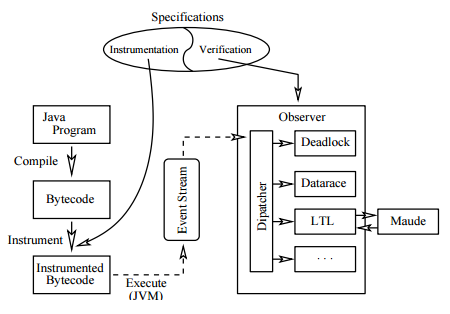
\includegraphics[width=100mm]{jpax.png}
\caption{JPaX Architecture (from \cite{havelund2001java})}
\label{img:jpax}
\end{center}
\end{figure}

JavaMaC \citep{kim2004java} is a ``run-time assurance system'' for Java programs while Mac means Monitoring and Checking. Its architecture is shown in Figure \ref{img:javamac}. Two definition languages are proposed: one for high-level specification which specifies required properties, another for low-level specification which defines the events and conditions. During the preparation, a ``filter'' and an ``event recognizer'' which are used to collect the necessary event traces are generated from the low-level specification, and a ``run-time checker'' is generated from the high-level spec. When running with the target program, events collected by the ``filter'' and ``event recognizer'' are sent to the ``run-time'' checker which is then responsible for the runtime verification work.

\begin{figure}[h]
\begin{center}
\centering
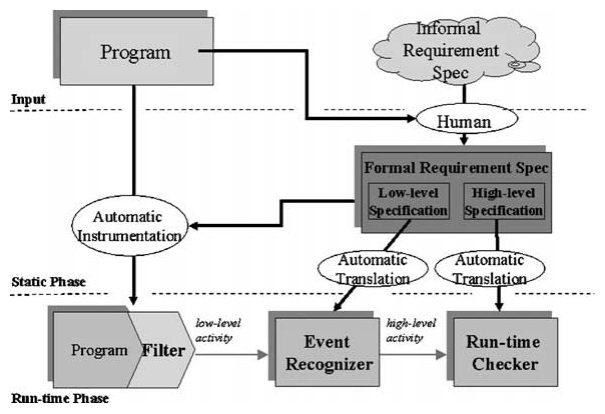
\includegraphics[width=100mm]{javamac.png}
\caption{MaC Architecture (from \cite{kim2004java})}
\label{img:javamac}
\end{center}
\end{figure}

\cite{d2005event} presents a logic named HAWK and its tools for RV of Java programs. HAWK is in fact built on EAGLE, another temporal logic which is considered more expressive \citep{barringer2004rule}. Although HAWK is event-based in contrast to state-based EAGLE, HAWK specifications are translated to EAGLE monitors. As Figure \ref{img:eagle} describes, during program execution, the EAGLE state is updated by instrumented program which then notifies the EAGLE observer. After that, the observer assesses the formul\ae{} in the current state to produce a result. 

\begin{figure}[h]
\begin{center}
\centering
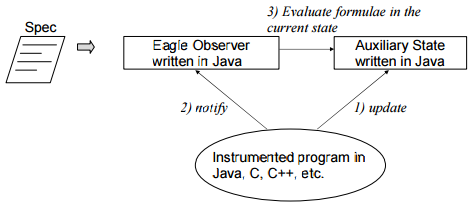
\includegraphics[width=100mm]{eagle.png}
\caption{Eagle Architecture (from \cite{d2005event})}
\label{img:eagle}
\end{center}
\end{figure}

Temporal Rover \citep{drusinsky2000temporal} is a commercial runtime verification tool based on LTL and MTL (Metric Temporal Logic). The specification code of Temporal Rover is inserted into the source code of Java, C, C++ or HDL and then converted into a compilable source file of corresponding language. A Temporal-Rover runtime verification system normally has two parts: host and target. The host is responsible for the verification while the target performs the computation of propositional formul\ae{} and sends back the results to the host via serial port, RPC or other customizable protocol.

Each of the frameworks discussed above hardwires a different specification formalism, which suggests that a general specification formalism serving all purposes does not exist. To be more expressive and generic, \cite{chen2007mop} introduced customizable and extensible ``logic-plugins'' in their runtime framework MOP and designed its architecture shown in Figure \ref{img:mop} with two layers: one is called ``language clients'' which support different programming languages, while another is ``logic repository'' which includes and manages various ``logic-plugins'' to support different specification formalisms, such as : Linear Temporal Logic (ltl), Finite State Machines (fsm), Extended Regular Expressions (ere), Context Free Grammars (cfg) and String Rewriting Systems (srs).

\begin{figure}[h]
\begin{center}
\centering
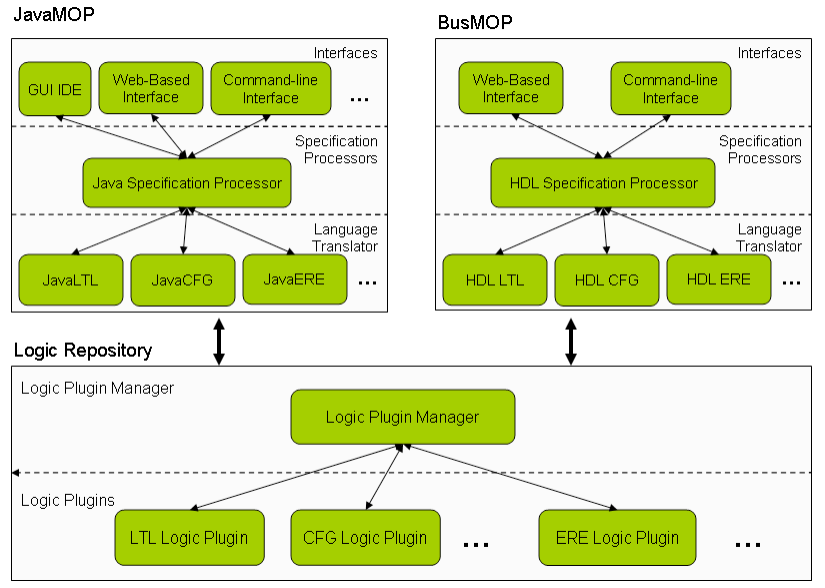
\includegraphics[width=130mm]{mop.png}
\caption{MOP Architecture (from \cite{chen2007mop})}
\label{img:mop}
\end{center}
\end{figure}

Besides the frameworks presented above, there are also lots of other frameworks invented for their corresponding requirements or specific temporal logics. Comparing these frameworks, we can find that they have their specialties as well as they share some common characters. For example, nearly all frameworks support online monitoring mode, Java programming language and network communication perhaps because these features are the most popular requirement in industry. Temporal Rover is a commercial RV framework, so it has to support more programming languages and supply more data collection options in order to expand its marketing. MOP was designed to be extremely general, resulting that most components can be changed or separately optimized.
